\section{Concorrenza}

La concorrenza è un concetto fondamentale nell'ambito
dello sviluppo software, si riferisce alla capacità
di eseguire più attività contemporaneamente.
Questo è particolarmente importante in applicazione
che devono gestire molteplici operazioni in parallelo
come ad esempio un server web, applicazioni di
elaborazione dati.

La concorrenza consente a un programma di sfruttare appieno
le risorse disponibili, aumentando l'efficienza e migliorando
le prestazioni complessive.
Inoltre, permette di creare sistemi più reattivi e
scalabili, in grado di gestire un numero crescente di
richieste senza compromettere le prestazioni.

In generale, la gestione della concorrenza può essere complessa
e soggetta a errori o comportamenti indeterminati, infatti,
più processi o thread possono interagire tra loro in modo
imprevedibile, essendo così costretti a usare tecniche di
locking in concomitanza di memoria condivisa trà più thread.

Nel contesto di Elixir, la concorrenza è un concetto centrale
e viene gestita attraverso il modello di programmazione
basato su processi leggeri, tutti isolati tra loro con il proprio
stack ed il proprio heap.

% ------------------------------------------------------

\subsection{La concorrenza in Beam}

La concorrenza gioca un ruolo chiave per un software
che vuole essere altamente responsivo.
La concorrenza è raggiunta nella piattaforma Erlang
con il concetto di Processo, per processo non si intende
il processo del sistema operativo, ma processo della
VM, chiamato processo e non thread in quanto non
condividono memoria tra di loro e sono completamente
isolati.

Un server tipico deve gestire migliaia di richieste, e
gestirle concorrenzialmente è essenziale per non far
rimanere in attesa il client. Quello che si vuole è
gestirli parallelamente il più possibile sfruttando
più risorse della Cpu disponibile.
Quello che fa la macchina virtuale per noi è permetterci
la scalabilità, più richieste allora più risorse da allocare.

Siccome il processo è isolato, un errore in una richiesta
ad esempio può essere localizzato senza avere impatto
sul resto del sistema, così creando anche un sistema robusto
agli errori.

In Beam due processi sono eseguiti concorrenzialmente e
se sono disponibili due Cpu core, forse sono eseguiti anche
in parallelo, la gestione della concorrenza è gestita
dalla macchina virtuale come in figura \ref{fig:concorrenza_beam}
in un computer dual core.


\begin{figure}[!htp]
    \centering
    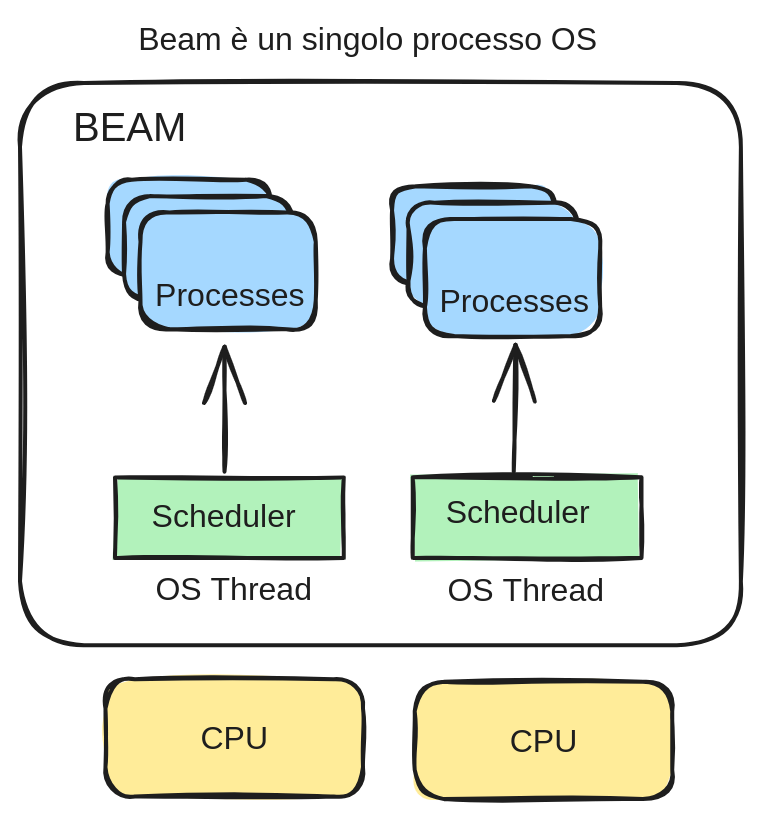
\includegraphics[keepaspectratio=true,scale=0.25]{images/beam_concurrency.png}
	\caption{Concorrenza nella VM Beam \cite{elixirInAction5}}
  	\label{fig:concorrenza_beam}
\end{figure}

In Beam i processi sono entità leggere e sono gestiti
dalla macchina virtuale usando il proprio scheduler.
In dettaglio, la VM alloca di default uno scheduler per ogni
core logico disponibile, 


%--------------------------------------------------------------

\subsection{Concorrenza basata su attori}

Elixir usa un modello di concorrenza basato su attori,
Gli attori sono entità di elaborazione indipendenti
che eseguono operazioni in modo asincrono, questi attori
non sono altri che  processi che vengono identificati
attraverso un \textbf{PID} univoco.
Gli attori sono isolati l'uno dall'altro e
comunicano solo attraverso lo scambio di messaggi,
questo scambio avviene attraverso
dei canali di comunicazione detti \textbf{"mailbox"}.
Ogni processo ha una propria mailbox dove avviene la
ricezione del messaggio.

Conoscendo il PID di un processo può avvenire la comunicazione
attraverso la primitiva fornita dal linguaggio.

Un processo può essere creato tramite la primitiva \textbf{spawn/1},

\begin{lstlisting}[language=elixir, caption={Creazione processo},captionpos=b,
	label={lst:creazione_processo}]
iex(1)> pid = spawn(fn -> IO.puts("Hello") end)
Hello
#PID<0.114.0>
\end{lstlisting}